\section{Introduction}\label{sec:intro}

% batching is important
Transaction processing is a fundamental aspect of database functionality, and improving OLTP system performance is a key research goal. The throughput of OLTP systems can be increased through \emph{batching} of operations; specifically, some component can buffer a number of operations as they arrive then \changed{process} them as a group \cite{friedman1997packing,debrabant2013anti,hagmann1987reimplementing}.
Batching can improve system performance for several reasons. First, at the networking layer, it increases the communication efficiency by packing messages~\cite{ding2015centiman,friedman1997packing}. Second, it amortizes the cost of system calls by condensing multiple requests into a single one, as in group commit~\cite{debrabant2013anti,hagmann1987reimplementing}. Third, it reduces the number of requests by discarding duplicate or stale requests, such as writes to the same record~\cite{faleiro2014lazy}. All of those are optimizations based on low-level techniques, and they do not take the semantics of the system into account.

% our proposal at a high level: batching at higher level for OCC 
We propose to embrace semantic batching as a core design principle throughout transaction execution for OLTP systems with optimistic concurrency control (OCC)~\cite{kung81tods}.
OCC is a popular concurrency control protocol due to its low overhead in low-contention
settings~\cite{adya97podc, baker11cidr, bernstein2015optimizing,bernstein11cidr,
bernstein11vldb, corbett12osdi,warp, patterson12vldb,peng10osdi,larson2011high}. However, it has been shown that OCC
wastes resources when conflicts are frequent~\cite{agrawal1987concurrency}. We
show how semantic batching (and associated reordering of transactions) can reduce the number of conflicts, improve
throughput and latency, and allow us to use OCC with higher-contention workloads.


Figure~\ref{fig:occ_arch} shows a prototypical architecture of a modern, loosely coupled OCC-based transaction processing system with a separation of compute and storage such as Centiman~\cite{ding2015centiman}. 
The system consists of three components: processors, storage, and one or more validators. External clients issue transactions to the system. On arrival into the system, each transaction is assigned to a processor and enters its \emph{read} phase. The processor sends read requests to the storage, executes the transaction, and performs writes to a local workspace. After it has processed the transaction, it sends information about the transaction's reads and writes to the validator. 
The transaction now enters the \emph{validation} phase, where 
% In OCC with \emph{backward validation}, 
the validator checks if there are conflicts with a previously committed transaction. \eat{, and makes a``success'' or ``failure'' validation decision.}
%jg01: We need a citation after ``decision.''
One example of a conflict that would fail validation is a \emph{stale read}. Suppose a transaction $t$ reads an object $x$, and a second transaction
$t'$ writes to the same object after $t$'s read. If $t'$ commits before $t$, $t$
has a conflict, since it should have read the update $t'$ made to $x$. Hence, $t$ must fail validation. 
If a transaction passes validation, the processor sends its writes to the storage; this is the \emph{write} phase. Otherwise, the processor aborts and restarts the transaction.

% why OCC for batching
%The architecture of 
OCC 
%with backward validation
presents unique opportunities for batching because the final serialization order of transactions is only decided at commit time in the validator. 
% batching at processor
There are three opportunities to apply semantic batching. The first is the processor in
the transactions' read phase, where transaction requests can be batched before
execution. Recent work in the context of locking-based protocols batch transactions 
and serialize them before execution to reduce overhead~\cite{faleiro2014rethinking,mu2014extracting,thomson2012calvin}; 
these techniques can be adapted and applied in OCC as well.

% batching at validator
The second possible place is the validator. The validator can batch validation requests and then select 
a validation order that reduces the number of conflicts and
aborts. Assume again two transactions $t$ and $t'$ where $t$ reads $x$,
and $t'$ writes $x$ after $t$'s read. Without batching, if $t'$ arrives at
the validator before $t$ and commits, $t$ will fail. With
batching, if $t$ and $t'$ are in the same validation batch, 
we can serialize $t$ before $t'$ (assuming no other dependencies between the transactions), 
and we can commit both transactions without any aborts.

% batching at storage
Third, batching can be done at the storage level. This affects
already-validated transactions in their write phase as well as transactions
still in their read phase. The storage can buffer read and write requests into
joint batches as they arrive. If a batch contains read and write requests for
the same object, the system can apply all the writes first in their serialization
order and then process the reads. Prioritizing writes over reads is always
optimal as this reduces the number of aborts later in the validator as much as possible. This is
because OCC reads come from uncommitted transactions, while writes come from
validated transactions that will commit soon. Thus, if the storage schedules a
pending read before a pending write on the same object, the reading transaction
will see a stale value and is guaranteed to fail validation. 

% drawback of batching
%Batching at these three levels in the system reduces aborts due to conflicts, and thus can increase throughput.\eat{However, it may also increase latency.}

\begin{figure}[t]
 \centering
 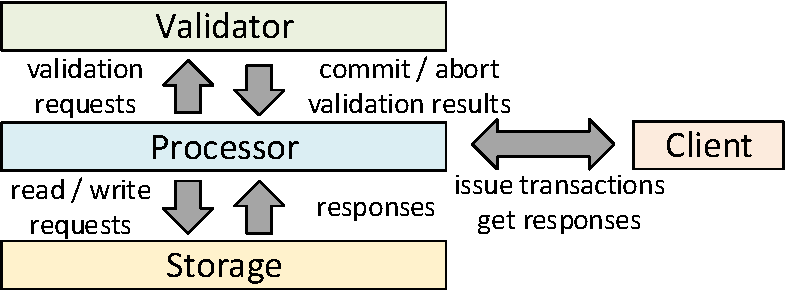
\includegraphics[width=0.9\columnwidth]{figures/arch.pdf}
 %\vspace{-.5em}
 \caption{OCC system architecture}
% \vspace{-1em}
 \label{fig:occ_arch}
\end{figure}


% contribution
{\bf Contributions of this paper.}
We explore the benefits of transaction batching and operation reordering in OCC with backward validation, with a focus on storage and validator batching. 
\cut{Our system design is best suited for integration with an in-memory versioned key-value store, as we require the ability to customize the validation logic. }
%Previous work on the Centiman system\cite{ding2015centiman} proposed a loosely coupled architecture for OCC on top of key-value stores. The system we present here follows Centiman's architecture and enhances its design with batching and reordering.
%\begin{itemize}
% contribution 1: system design
%\item 
%\begin{itemize}
%\item 

$\bullet$ Our first contribution is to show how to integrate batching and reordering throughout the lifetime of a transaction to enhance OCC-based protocols. We analyze the reasons for conflicts and aborts at each stage of a transaction's life cycle, and develop techniques to reduce these aborts through semantic batching.
We introduce intra-batch storage reordering and
intra-batch validator reordering, and we show that selecting the
optimal transaction ordering at the validator batch is NP-hard.
(Section \ref{sec:overview}).


$\bullet$ Our second contribution is 
two practical classes of greedy algorithms for validator reordering 
that balance abort rates and reordering overheads.
%These algorithms produce good orderings in practice, and they are fast to
%use in a real system. 
We also extend these algorithms to weighted versions that can
incorporate policies such as transaction priorities (Section \ref{sec:valbatching}).


% contribution 3: parallel validation
%\item 
$\bullet$ Our third contribution is a design that reduces the amortized overhead of validation through parallelism. The parallelization is achieved with a three-stage pipeline, where the stages are batch preparation, transaction reordering, and transaction validation. Each of these stages can be further parallelized to allow concurrent processing (Section \ref{sec:parallel}).

% contribution 4: experiment
%\item 
$\bullet$ In a detailed experimental study of the impact of storage and validator batching in a prototype system, as well as on top of a commercial database system, we show that batching and reordering always increases transaction throughput and, surprisingly, also reduces transaction latency, especially the tail latency. For workloads with high data contention, batching and reordering can improve the throughput by up to a factor of 3.1x and can reduce the average transaction latency by up to 82\% for a micro benchmark and the Small Bank Benchmark~\cite{alomari2008icde} (Section \ref{sec:experiments}).
%\end{itemize}

\eat{
%paper organization
The remainder of the paper is organized as follows. In Section~\ref{sec:background}  we review OCC with backward validation. In Section~\ref{sec:overview} we discuss challenges, opportunities and techniques for storage and validator batching. In Section~\ref{sec:validator_reordering}, we introduce our algorithms for transaction reordering as well as parallelization at the validator. In Section~\ref{sec:experiments}, we present an extensive evaluation of our system. We discuss related work in Section~\ref{sec:relwork} and conclude in Section~\ref{sec:conclusion}.
}
